\documentclass[11pt]{article}
\usepackage{geometry,tabularx,booktabs,float}                % See geometry.pdf to learn the layout options. There are lots.
\geometry{letterpaper}                   % ... or a4paper or a5paper or ... 
%\geometry{landscape}                % Activate for for rotated page geometry
%\usepackage[parfill]{parskip}    % Activate to begin paragraphs with an empty line rather than an indent
\usepackage{graphicx}
\usepackage{amssymb}
\usepackage{epstopdf}
\DeclareGraphicsRule{.tif}{png}{.png}{`convert #1 `dirname #1`/`basename #1 .tif`.png}

\title{A Usability Study Comparing iTunes and Spotify}
\author{Juan S. Carrillo}
%\date{}                                           % Activate to display a given date or no date

\begin{document}
\maketitle
\section{Introduction}
For this study our group wished to compare the usability of two music services, iTunes and Spotify. For the purpose of our study we only included the desktop version of Spotify, since iTunes does not have a mobile version. The focus of our study is to determine which of the two music services has better usability.
\section{Background}
\subsection{Metrics}
Our study focuses on the efficiency, rate of errors, and satisfaction of the user with the two music services. We study the \textit{efficiency} of the music service by measuring the time it takes for the user to perform a given task. When we test for efficiency, we only consider users that are already familiar with the music service. In this way, we are sure that the user is not wasting time becoming familiar with the system itself; all the work on the part of the user is focused on completing the task at hand. When we measure the \textit{rate of errors} while using the programs, we analyze how many errors are made on the part of the user, that is, when they perform an action that has unintentional results. We quantify these by simply counting how many errors were committed. In this study we found that people that took a long time to finish a task were hindered by one significant error rather than a series of minor errors.  We also surveyed the \textit{satisfaction} of the users. We simply asked the users to report on a numeric scale how satisfied they were with the ease of performing the given tasks or with the music service and we also asked how satisfied they were with the music service as a whole.
\subsection{Tasks}
For the study we wanted to come up with tasks that were complex enough that the user would have to perform two or more actions in order to accomplish the task but at the same time were familiar enough to the user so that they understood the task. We choose the following tasks:
\begin{itemize}
    \item \textbf{Creating an empty playlist}: The user was asked to create an empty playlist with the title "Hello World".
    \item \textbf{Creating a radio station based on a given artist}: The user was asked to create a radio station based on the artist Ti\"{e}sto and play it.
    \item \textbf{Looping a playlist}: The user was asked to play a playlist and set it to loop indefinitely, i.e., the music service would play all the songs in the playlist and when it had gone through all the songs in the playlist it would iterate through the playlist again and continue playing the songs in the list. The user was allowed to use a playlist that they had already created beforehand or were given time to create a playlist in order to finish the task.  
\end{itemize} 

Each of these tasks is familiar to most users and required more than one action to complete, i.e., pressing a button and writing out the title of a playlist. These tasks are also possible in both systems. Since iTunes is a media player while Spotify is a music streaming service, we had to take care to create tasks that were possible in both systems. 
\section{Procedure}
We created a spreadsheet using Google Docs and created a form that would record all the data from the survey on the sheet. Each member of our group recorded the data on the form for an individual participant. The form contained the following fields:
\begin{itemize}
    \item The service that the user was testing 
    \item Whether or not the user had previously used the music service 
    \item How long had the user been using the music service 
    \item How the user rated themselves on how familiar they were with the music service
    \item How the user rated their proficiency with computers
    \item The time it took to the user to complete a given task
    \item How many errors, if any, were committed while completing each task
    \item A brief qualitative description of the errors, if any
    \item Any additional notes on any given task
    \item Satisfaction with the ease of the given task
    \item Overall satisfaction with the music service
\end{itemize}  
For the question concerning how familiar they were with the music service, the user was asked to rank themselves from 1 to 10, 1 being very unfamiliar and 10 being very familiar with the service. Similarly, the user was asked to rate their proficiency with computers on a scale from 1 to 10, 1 being not very proficient and 10 being very proficient.

We allowed the users to use their personal computer for the survey in order to make sure the users did not take longer because they were using an operating system they are unfamiliar with. % JD: Good variable to eliminate, especially for efficiency.
Also, there is no significant difference between the application windows across operating systems, as seen in Figures ~\ref{fig:spotify_view} and ~\ref{fig:iTunes_view}. Note that the application windows are stacked in the order of Mac and Windows.

\begin{figure}[H] %  figure placement: here, top, bottom, or page
   \centering
   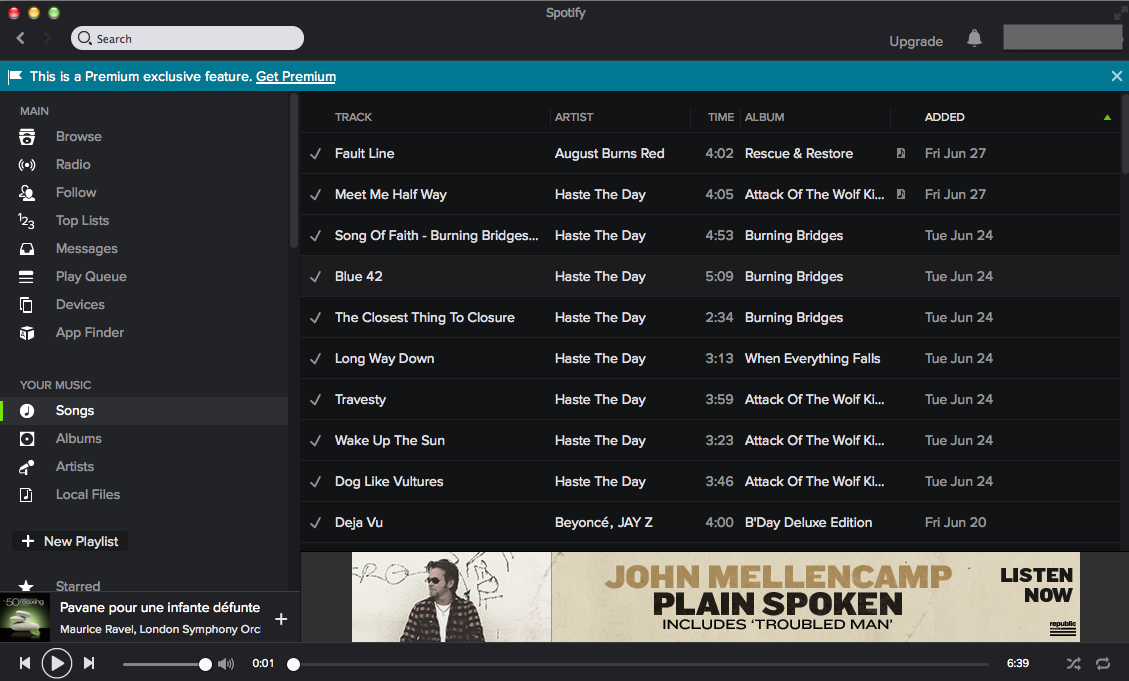
\includegraphics[width=3in]{spotify_mac.png}       
   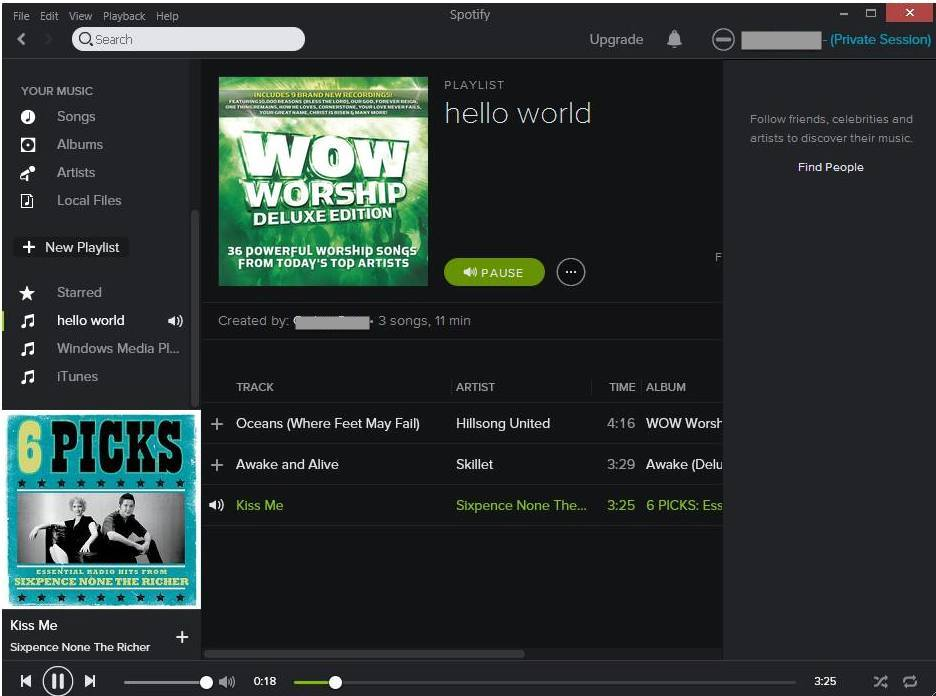
\includegraphics[width=3in]{spotify_pc.jpg} 
   \caption{Spotify Desktop Application View}
   \label{fig:spotify_view}
\end{figure}

\begin{figure}[H] %  figure placement: here, top, bottom, or page
   \centering
   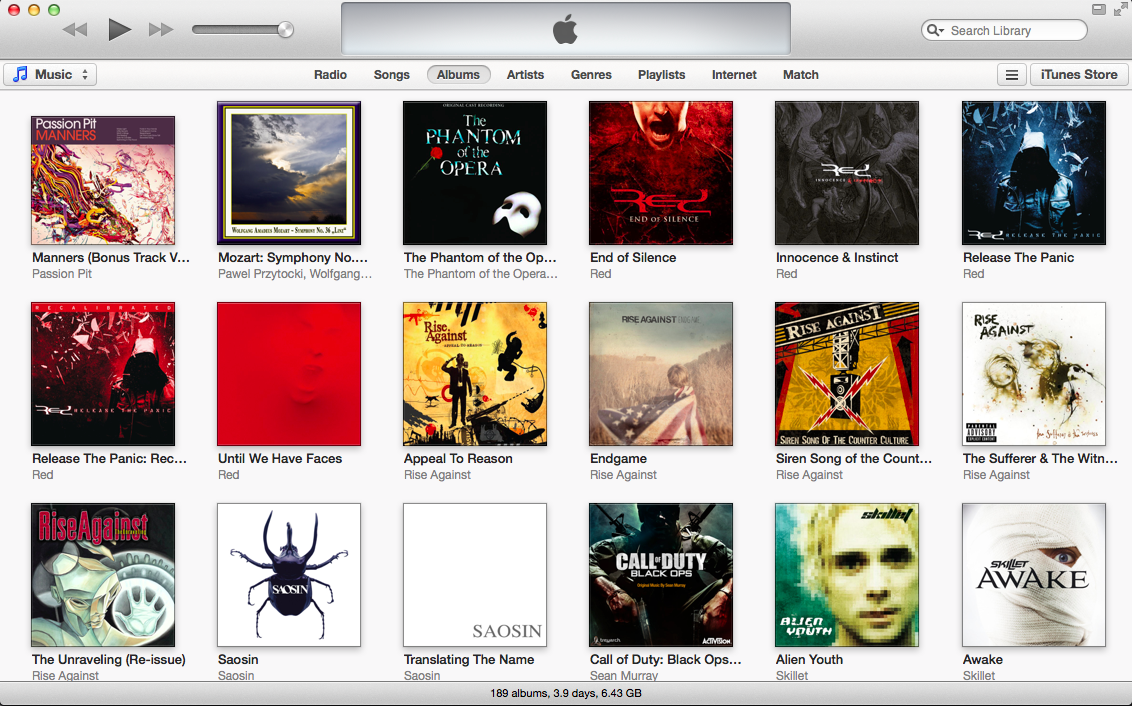
\includegraphics[width=3in]{iTunes_mac.png}       
   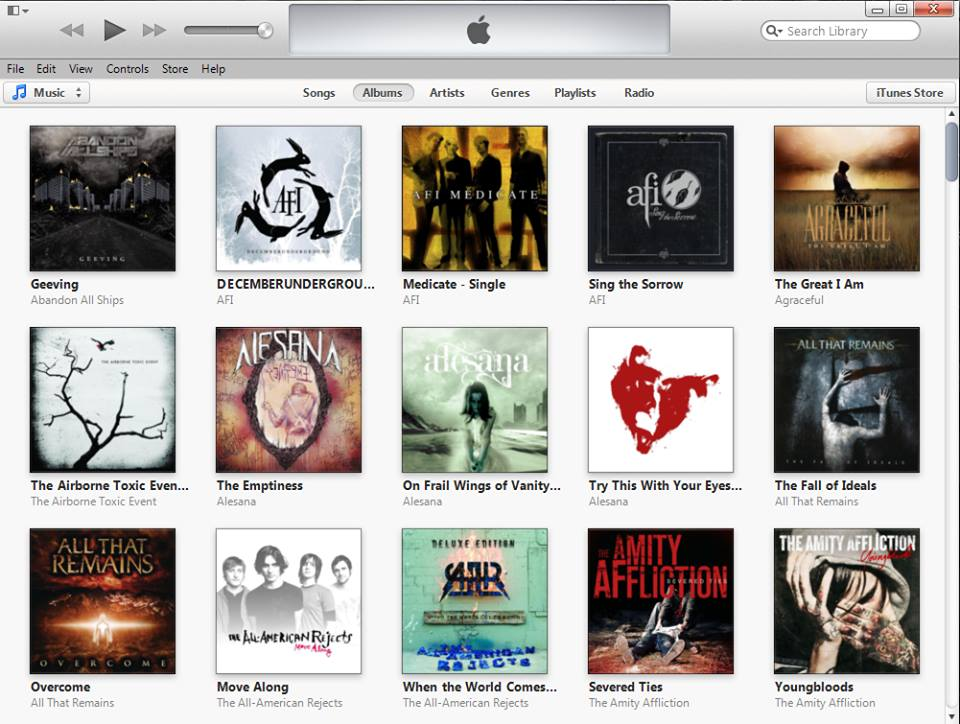
\includegraphics[width=3in]{iTunes_pc.jpg}
   \caption{iTunes Application View}
   \label{fig:iTunes_view}
\end{figure}

 
At the beginning of the survey we collected information for the first five fields. After collecting the preliminary data, we explained the task to the participant and then timed how long it took for each participant to complete the given task. We also made note of any errors committed by the user. In between each task we asked the participant to report their satisfaction with each task on a scale of 1 to 10, 1 being very unsatisfied and 10 being very satisfied. We also recorded any additional comments provided by the user, if relevant. At the end of the survey we asked the user to rate their overall satisfaction with the music service on a scale of 1 to 10, 1 being very unsatisfied and 10 being very satisfied.
\section{Results}
When looking at the results, I placed most of the importance on rate of errors and learnability
% JD: Learnability???   O_o
than satisfaction. I do this because I believe that satisfaction is a direct result of the other two metrics; if the system is very learnable or if the rate of errors is low then the satisfaction of the users with the system will be high. Thus, I base my assessment of the system more on the metrics of learnability and rate of errors, while using satisfaction to confirm the results from the other metrics.
% JD: You wrote "learnability" a couple more times...so now I'm sure it's not a typo.
\subsection{Participants}
We had 15 examinations, 8 for iTunes and 7 for Spotify. Some of the users participated in the survey twice, testing one service and then the other.  All participants that tested iTunes were already familiar with iTunes. Of the 7 participants who tested Spotify only 4 were prior experience with Spotify. The average self-assessed proficiency of the participants was about 7.46, with a standard deviation of 1.73, meaning that users considered themselves to be proficient at using a computer. 


\subsection{Experience and Satisfaction}

\begin{figure}[H] %  figure placement: here, top, bottom, or page
   \centering
   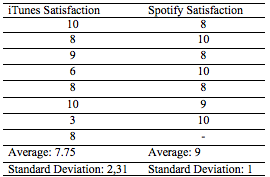
\includegraphics[width=2.4in]{satisfaction_.png}       
   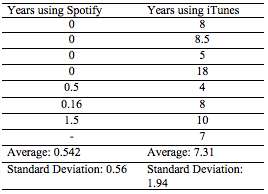
\includegraphics[width=2.22in]{times_used.png} 
   \caption{User Satisfaction and Experience}
   \label{fig:satisfaction}
\end{figure}

All the people who tested iTunes were already familiar with the service. Looking at Figure~\ref{fig:satisfaction}, we see that on average, those participants that had used iTunes had been using it for about 7 years. In contrast, three out of the seven participants for Spotify had no previous experience with Spotify. As a result of this and the small sample size, the average participant had only 6 months of experience with Spotify. Also, no user had more than 18 months of experience with Spotify. The average is not % JD: Cutoff sentence?  Leftover that should be deleted?
The average satisfaction with the system was 7.75, with a standard deviation of 2.31, which means that users were overall satisfied with the system. It can be noted that one user in particular rated their satisfaction with iTunes at a 3, and the next lowest score was a 6. Due to the small sample size, the user's score greatly lowered the average satisfaction for iTunes. It can also be noted that the user took 1 minute and 30 seconds on one of the tasks, and their overall satisfaction with iTunes may be attributed to the relatively long time it took the participant to complete that task. On the other hand, those who participated with Spotify reported on average a satisfaction of 9. The data we collected suggests that overall users have greater satisfaction with Spotify.

\subsection{Creating the Playlist}

\begin{figure}[H] %  figure placement: here, top, bottom, or page
   \centering
   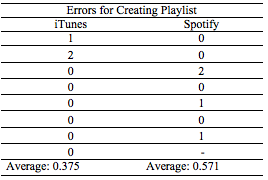
\includegraphics[width=2.4in]{errors_playlist.png}       
   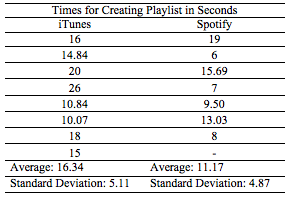
\includegraphics[width=2.4in]{times_playlist.png} 
   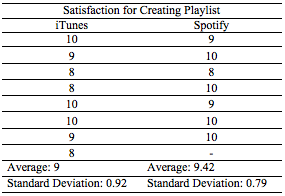
\includegraphics[width=2.4in]{satisfaction_playlist.png} 
   \caption{Times, Errors, and Satisfaction Creating a Playlist}
   \label{fig:playlist}
\end{figure}

Users were significantly faster using Spotify when creating the playlist, despite also committing more errors while using Spotify. Most users noted  that it was easy to create a playlist in Spotify because there is a widget on the left-hand side with a plus sign labeled New Playlist. Most errors involved misspelling the title of the playlist, "Hello World". Although those using iTunes varied in their approaches to creating the playlist, i.e., using keyboard shortcuts or clicking on buttons, they were on average much slower than when the participants used Spotify. It is to be noted that one of the users complained that iTunes is constantly changing its layout, making the users remember new ways to create a playlist. I speculate that the change of the layout causes users to waste time trying to use their usual approach and realizing that the change of the layout changes the way they must create a playlist. We can see that Spotify had a higher satisfaction for this task than iTunes. 

\subsection{Creating the Radio Station}

\begin{figure}[H] %  figure placement: here, top, bottom, or page
   \centering
   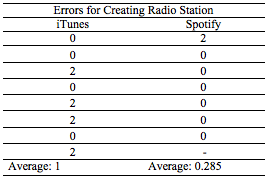
\includegraphics[width=2.4in]{errors_radio.png}       
   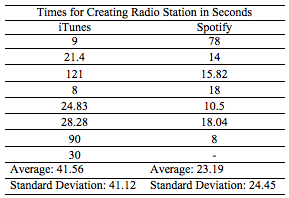
\includegraphics[width=2.4in]{times_radio.png} 
   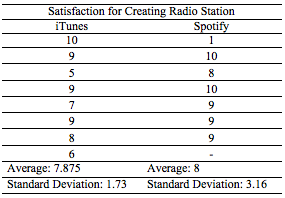
\includegraphics[width=2.4in]{satisfaction_radio.png}    
   \caption{Times, Errors, and Satisfaction for Creating Radio Station}
   \label{fig:radio}
\end{figure}

In both music services there were users that took a very long time to figure out how to create a radio station based on an artist. However, Spotify again proved to be faster as users took on average 23.19 seconds complete the task, while completing the same task on iTunes took on average 41.56 seconds. Since the standard deviation for Spotify is much smaller than the one for iTunes, it also demonstrates that the distribution of times is also much tighter than that of iTunes. It is important to note that there were many errors when using iTunes. All of them involved users being unable to find the method to create a radio station based on an artist. However, on Spotify users usually looked up the artist and then looked for ways to create a radio station from there. I speculate that the reason that users were much faster on Spotify is that there were two ways of creating a radio station: finding the artist and creating a station, or going to the radio button and then clicking "Create New Station", which prompted the user to type in the name of the artist. However on iTunes the option of looking up the artist and then creating a radio station was not available. Here, I believe the deciding factor was that there was more than one way to do the same thing in Spotify. Again, we see that Spotify had a higher satisfaction than iTunes.

\subsection{Looping the Playlist}

\begin{figure}[H] %  figure placement: here, top, bottom, or page
   \centering
   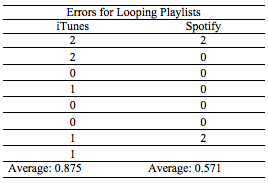
\includegraphics[width=2.4in]{errors_loop.png}       
   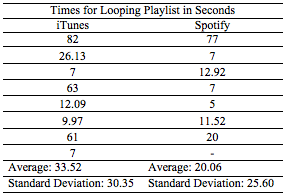
\includegraphics[width=2.4in]{times_loop.png}
   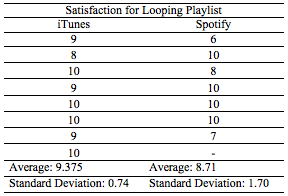
\includegraphics[width=2.4in]{satisfaction_looping.png}        
   \caption{Times, Errors, and Satisfaction for Looping the Playlist}
   \label{fig:loop}
\end{figure}

This task was unusual in the sense that the music service that had the least amount of errors and took the least amount to complete had the lower satisfaction. One average it took 20 seconds to loop a list in Spotify, while it took 33 seconds to perform the same task on iTunes. Also, there were fewer errors on Spotify than on iTunes. However, there were two users who gave Spotify a satisfaction of 6 and 7, which is lower than the any satisfaction score given to iTunes. Both of these users were unable to get the playlists to loop right away; one of the users couldn't find the icon to loop and the other did not to play the playlist first, which is necessary to activate the loop button. I believe that the reason for these low scores is that the users were disappointed at not being able to find the icons right away. Seeing as how this case goes against the pattern established by the previous two tests, where the music service that required the least amount of time and had less errors had higher satisfaction, it prompts the author to want to gather a larger sample size in order to draw a good conclusion. % JD: What happens when you remove those two outliers?
%\subsection{}
\section{Analysis}
\subsection{Efficiency}
It is difficult to measure the efficiency for all the tasks evenly. We certainly cannot compare the efficiency of one system to the next because all participants were already familiar with iTunes, while not all participants were previously acquainted with Spotify. The sample size for Spotify is too small to consider the efficiency of Spotify.
% JD: True, that does mess with the numbers a bit.  Aside from increasing the sample size,
%     you could also have given everyone "free time" with both apps to ensure that they
%     felt sufficiently proficient at both of them.
\subsection{Learnability}
I believe that Spotify had better learnability than iTunes.
% JD: Hrrrm; your introduction talked about efficiency; and with the collective user experience
%     with iTunes you really can't use learnability.  In a way, you are closer to efficiency
%     here than learnability.
This becomes obvious in the task that asked users to create a radio station based on an artist. I attribute Spotify's success because they had two different methods to do the same thing, and both seem intuitive given the model of Spotify. As a streaming service, Spotify gives users access to music they haven't purchased, unlike iTunes which serves as a media library to organize the music files they had saved on their computer. Since Spotify allows users to music from almost any artist, it is natural for a user to search an artist on Spotify's search bar. From the artist's page the user has the option to create a radio station based on the artist by clicking a button with ellipsis and then selecting ``Start Artist Radio.'' Spotify also had a button on the side bar labeled Radio. If this button is clicked the view changes to the most recent radio station. This view has a button on the upper right hand corner labeled ``Start New Station.'' After clicking this button the user can input an artist name into the dialog box and immediately start a new radio station based on that artist. So while this task was the one that most users were unfamiliar with, and most, if not all, users had to figure out how to complete this task for the first time regardless of the platform. It is difficult to measure the learnability as easily with the other two tasks. Most users are already familiar with the action of creating a new playlist; most of the errors in this task involved mistyping the name of the playlist. 

Since all the iTunes users have had years of experience with the media player, it is safe to consider that they were all familiar with the task of creating a playlist. On the other hand, almost half of the users for Spotify had never used Spotify before. For Spotify, then, creating a new playlist was more of a learnability issue while for iTunes is was more of an efficiency issue. As previously stated, we have a rather small sample size, but it is interesting to note that beginner Spotify users take about the same time that an experienced Spotify user would to create a new playlist. We can attribute this to Nielsen's principle of ``Speaking the user's language.'' Spotify has a button on the side of left hand side labeled ``+New Playlist.'' When a user wants to create a new playlist, they can easily recognize the button. iTunes is a little less straightforward in comparison, as it has a simple, small button labelled with a + sign.
% JD: You got the distinction between learnability and efficiency here, so it isn't clear why
%     the distinction seems more muddled elsewhere in the paper.
%
%     Also, yes, good recognition that the explicit inclusion of the word "Playlist" in Spotify
%     may very well have been a factor in its time advantage.


\begin{figure}[H] %  figure placement: here, top, bottom, or page
   \centering
   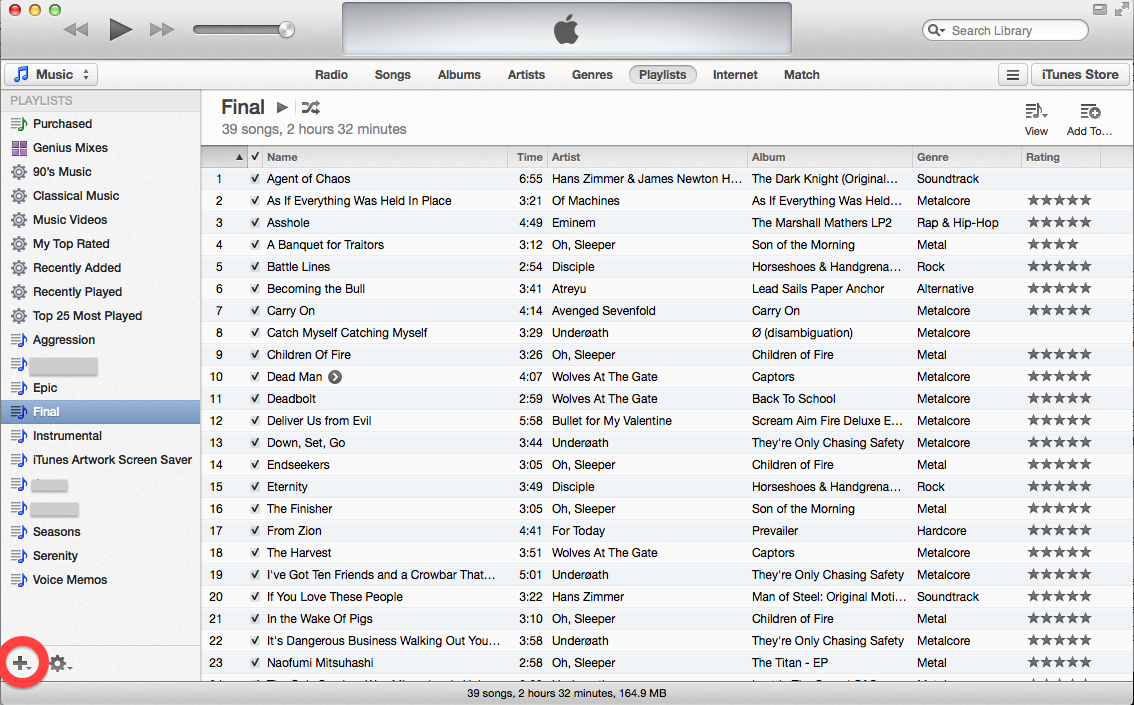
\includegraphics[width=5.5in]{iTunes_new_playlist.png}
   \caption{iTunes New Playlist Button in Red}   
   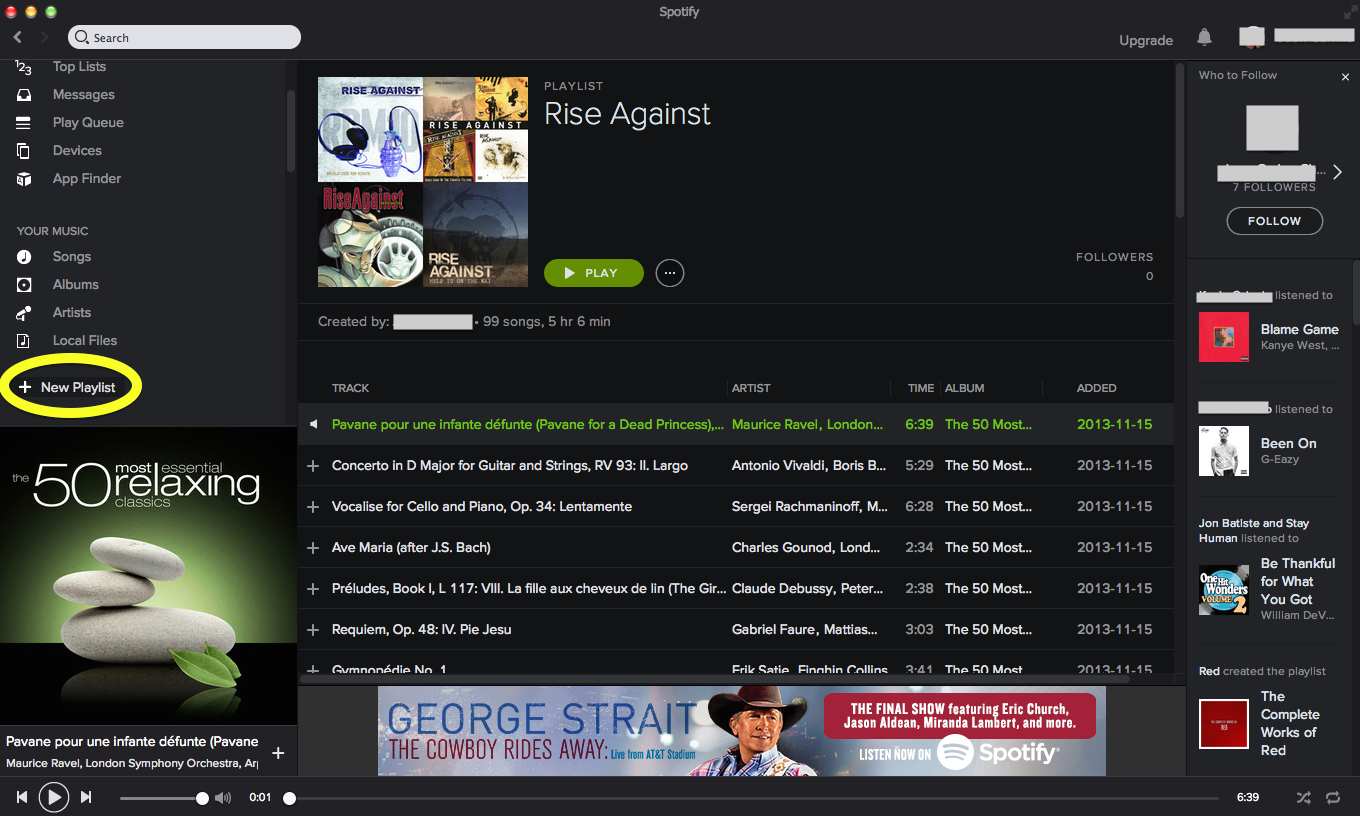
\includegraphics[width=5.5in]{spotify_new_playlist.png}
   \caption{Spotify New Playlist Button in Yellow}                                    
   \label{fig:iTunes_new_playlist}
\end{figure}

\subsection{Rate of Errors}
By analyzing the data, I see that Spotify has a lower rate of errors than iTunes. As previously stated, some of the users of iTunes noted that the media player has gone through several layout changes, which require iTunes users to relearn several tasks that they were familiar with. This contributes to the rate of errors because iTunes users might attempt to navigate to the command to create a new playlist and find it missing.
% JD: Does this exemplify a principle we've seen before?
During the release of iTunes 11, the layout of iTunes changed significantly \ref{iTunes11}, and so users had to get used to the new release. It is interesting to note that iTunes, as an established music service, did not do much better than Spotify, a much newer piece of music software. Considering that all participants of the iTunes surveys had years of experience on iTunes, they should have had a clear advantage over mundane tasks such as creating a playlist or looping a playlist. However, I believe that the recent changes in the iTunes interface cause iTunes to lose the advantage of having a familiar interface. This is in clear violation of one of the principles shared by several interaction design thinkers such as Tognazzini, Nielsen, and Shneiderman: consistency. The lack of consistency on iTunes caused it to be just as difficult to relearn an task in an old interface as it is to learn the same task in an unfamiliar interface, in this case Spotify.
% JD: Ah good, there it is :)

In fact, Spotify's default layout is more similar to that of the default layout of iTunes 10 (Figure~\ref{fig:iTunes10_and_spotify}) than that of iTunes 11. A shared characteristic is the presence of a vertical menu bar on the left hand side, called a ``source list'' on Spotify's Apps Design Guidelines and ``Sidebar'' on iTunes. It's interesting to note that iTunes 11.4 actually does have the Sidebar available, but users must manually change this by going into the View Tab. However, this is not the default layout of iTunes 11 and most users will prefer the layout to already be setup for them. The default Sidebar is one of the reasons that the change in iTunes 11 was controversial \ref{iTunes11}.

\begin{figure}[H] %  figure placement: here, top, bottom, or page
   \centering
   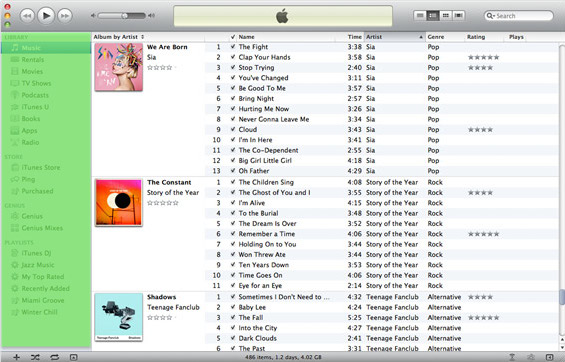
\includegraphics[width=2.5in]{iTunes10_sidebar.jpg}
   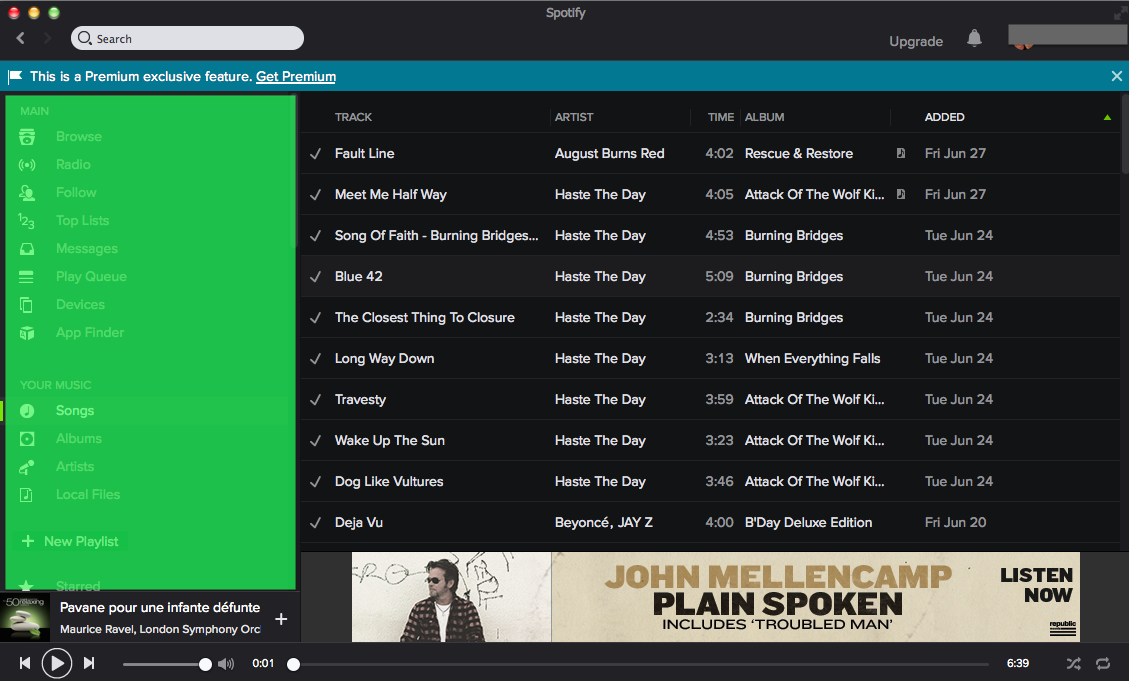
\includegraphics[width=2.5in]{spotify_mac_sidebar.png}
   \caption{Sidebar in iTunes and Source List on Spotify}                                    
   \label{fig:iTunes10_and_spotify}
\end{figure}

\subsection{Satisfaction}
Satisfaction was closely related to the previous two metrics. The higher satisfaction with the ease of a specific task usually went to the system that had lower rate of errors and higher efficiency or learnability. Even though this was not the case for the task of looping a playlist, Spotify was still able to come on top in terms of overall satisfaction, which is not surprising considering Spotify did better than iTunes in rate of errors and efficiency.

\section{Conclusion}
Both iTunes and Spotify are very popular. Any users that have an Apple device require iTunes to sync their media from their iTunes library to their device. % JD: Whaaaa.....?  This section looks unfinished.

\section{References}

% JD: As does this!

\end{document}  